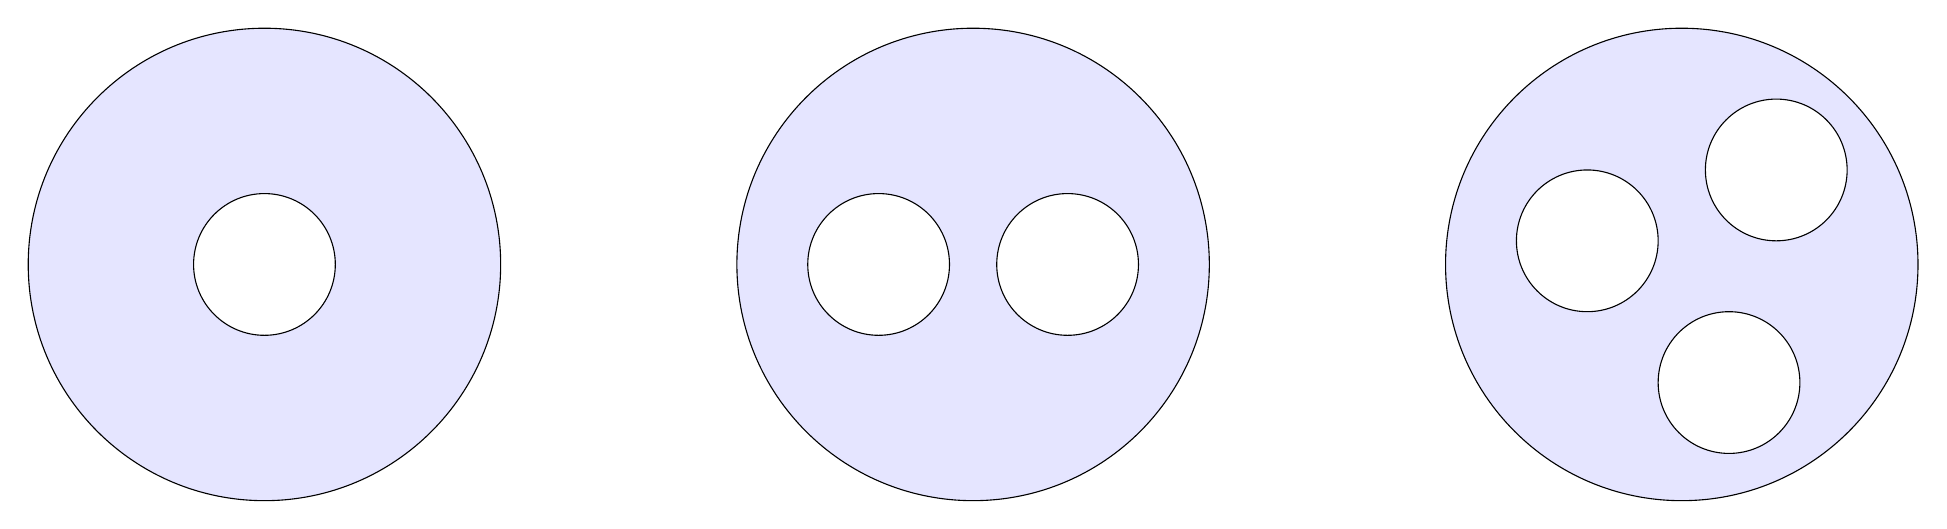
\begin{tikzpicture}[scale=3]
  % First circle with 1 hole
  \fill[blue!10] (0,0) circle(1);
  \draw (0,0) circle(1);
  \fill[white] (0,0) circle(0.3);
  \draw (0,0) circle(0.3);

  % Second circle with 2 holes
  \fill[blue!10] (3,0) circle(1);
  \draw (3,0) circle(1);
  \fill[white] (2.6,0) circle(0.3);
  \fill[white] (3.4,0) circle(0.3);
  \draw (2.6,0) circle(0.3);
  \draw (3.4,0) circle(0.3);

  % Third circle with 3 holes (like a face)
  \fill[blue!10] (6,0) circle(1);
  \draw (6,0) circle(1);
  \fill[white] (5.6,0.1) circle(0.3);
  \fill[white] (6.4,0.4) circle(0.3);
  \fill[white] (6.2,-0.5) circle(0.3);
  \draw (5.6,0.1) circle(0.3);
  \draw (6.4,0.4) circle(0.3);
  \draw (6.2,-0.5) circle(0.3);
\end{tikzpicture}